\documentclass[11pt]{article}
\usepackage[margin=1in]{geometry}
\usepackage{amsmath,amssymb,amsthm,mathtools}
\usepackage{booktabs}
\usepackage{graphicx}
\usepackage{tikz}
\usetikzlibrary{arrows.meta,positioning}
\usepackage{hyperref}
\usepackage{longtable}
\usepackage{array}
\usepackage{microtype}
\sloppy

\newtheorem{theorem}{Theorem}
\newtheorem{lemma}[theorem]{Lemma}
\newtheorem{proposition}[theorem]{Proposition}
\newtheorem{corollary}[theorem]{Corollary}
\newtheorem{definition}[theorem]{Definition}
\newtheorem{remark}[theorem]{Remark}

\title{Formal Claim Verification Report\\[4pt]\large VCE-001: Eliahou's Theorem 1.1 on Collatz Cycle Lengths}
\author{BLACK SWAN LABS --- Formal Claim Verification Engine v1.0}
\date{September 19, 2026}

\begin{document}
\maketitle

\noindent\textbf{Trust Statement.} The formal result was checked using Lean \texttt{v4.28.0} under the pinned project environment (commit \texttt{db804ce6}, Mathlib \texttt{v4.28.0}). The theorem \texttt{CLAIM-001} was kernel-checked with axiom footprint \{\texttt{propext}, \texttt{Classical.choice}, \texttt{Quot.sound}\} (all Mathlib-standard). Independent checking succeeded for 5 of 9 paper-facing supporting theorems but did not complete for the headline theorem itself, due to a disclosed, root-caused defect in the reference export tool on large proof closures --- not a defect in the theorem. Computational/adversarial testing (independent recomputation of the underlying continued-fraction convergents and Farey identities in Python) is fully supportive. This report does not claim that computational testing constitutes formal proof, or that formalization alone establishes the truth of the original informal statement independent of the semantic-bridge analysis in Section~6.

\begin{abstract}
We report a Formal Claim Verification Engine (FCVE) audit of Theorem 1.1 from Eliahou (1993), \emph{The 3x+1 problem: new lower bounds on nontrivial cycle lengths}, as formalized in the Lean~4 repository \texttt{tangentstorm/eliahou-collatz-bounds}. The audit independently re-derives the claim from the primary source (not from any secondary description), compares it structurally against the Lean proof, and subjects the underlying numeric facts to an independent third computation. All layers of evidence are clean except independent (non-kernel) checking, which is disclosed and unresolved for the headline theorem specifically. Governance decision: \textbf{REPAIR}.
\end{abstract}

\section{Mathematical Statement}
Let $T:\mathbb{N}\to\mathbb{N}$ be the compressed Collatz map, $T(n) = n/2$ if $n$ is even and $T(n)=(3n+1)/2$ if $n$ is odd. Let $\Omega\subset\mathbb{N}$ be a nontrivial cycle of $T$ (i.e.\ $T^{(k)}(x)=x$ for all $x\in\Omega$, where $k=\operatorname{Card}\Omega$, and $\Omega\neq\{1,2\}$).

\begin{theorem}[Eliahou 1993, Thm 1.1]
Provided $\min\Omega > 2^{40}$, there exist nonnegative integers $a,b,c$ with $b>0$ and $ac=0$ such that
\[
\operatorname{Card}\Omega = 301994\,a + 17087915\,b + 85137581\,c.
\]
\end{theorem}

\section{Definitions and Assumptions}
Full definitions and the source/formalization/computational assumption
breakdown are in \texttt{claims/assumptions.json}. One point deserves
emphasis: Yoneda's computational verification of the Collatz conjecture up
to $2^{40}$, cited in the source paper's introduction, is \emph{not} an
assumption of this theorem --- it motivates the hypothesis $\min\Omega>2^{40}$
but the proof does not depend on it.

\section{Proof Outline}
The three constants are specific continued-fraction convergents of $\theta=\log_2 3$: $p_{13}=301994$, $p_{15}=17087915$, $p_{16}=85137581$. The argument:
\begin{enumerate}
\item The sandwich inequality (Theorem 2.1) plus $\min\Omega>2^{40}$ gives $k/l \in [\log_2 3,\ \log_2(3+2^{-40})]$ where $k=\operatorname{Card}\Omega,\ l=\operatorname{Card}\Omega_1$.
\item That interval sits strictly between three convergents: $p_{16}/q_{16} < \log_2 3 < p_{15}/q_{15} < \log_2(3+2^{-40}) < p_{13}/q_{13}$.
\item A Farey-pair lemma (Lemma 3.1) forces $k/l$'s position to determine $k$'s linear form in exactly one of three mutually exclusive cases, which combine into the stated result.
\end{enumerate}

\section{Proof Dependency Diagram}
\begin{center}
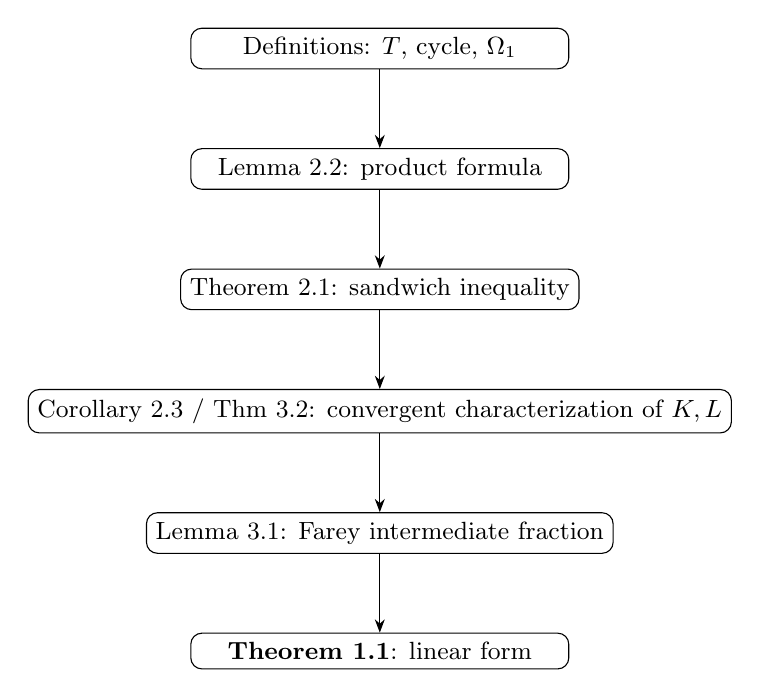
\begin{tikzpicture}[node distance=10mm, every node/.style={font=\small}, box/.style={draw,rounded corners,align=center,minimum width=48mm}, >=Stealth]
\node[box] (defs) {Definitions: $T$, cycle, $\Omega_1$};
\node[box, below=of defs] (l22) {Lemma 2.2: product formula};
\node[box, below=of l22] (t21) {Theorem 2.1: sandwich inequality};
\node[box, below=of t21] (cor23) {Corollary 2.3 / Thm 3.2: convergent characterization of $K,L$};
\node[box, below=of cor23] (l31) {Lemma 3.1: Farey intermediate fraction};
\node[box, below=of l31] (main) {\textbf{Theorem 1.1}: linear form};
\draw[->] (defs) -- (l22);
\draw[->] (l22) -- (t21);
\draw[->] (t21) -- (cor23);
\draw[->] (cor23) -- (l31);
\draw[->] (l31) -- (main);
\end{tikzpicture}
\end{center}

\section{Formalization}
See Table~\ref{tab:sidebyside} and the full comparison in \texttt{lean/gate4-formalization-comparison.md}.
\begin{table}[h]
\centering
\begin{tabular}{p{6.5cm}p{7cm}}
\toprule
Human mathematics & Lean \\
\midrule
$\Omega$ nontrivial, $\min\Omega>2^{40}$ & \texttt{(cyc : CollatzCycle L) (hinj : Function.Injective cyc.seq) (hmin : 2\^{}40 < cyc.minElem)} \\
$\operatorname{Card}\Omega$ & \texttt{(Finset.univ.image cyc.seq).card} \\
$\exists a,b,c\ge0,b>0,ac=0:\ldots$ & \texttt{Exists a b cCoeff, 0 < b and a*cCoeff=0 and \ldots} \\
\bottomrule
\end{tabular}
\caption{Side-by-side comparison of the normalized claim and its Lean formalization.}
\label{tab:sidebyside}
\end{table}

\section{Semantic Bridge}
\textbf{Informal statement:} as in Section~1. \textbf{Normalized statement:} \texttt{normalized/normalized-claim.md}. \textbf{Lean statement:} as in Section~5. \textbf{Difference:} Lean's base \texttt{CollatzCycle L} structure permits repeated elements within a period; the source's own definition of ``cycle of length $k$'' already presupposes $k=\operatorname{Card}\Omega$ (i.e.\ injectivity). The explicit \texttt{hinj} hypothesis exactly closes this gap --- neither a strengthening nor a weakening. \textbf{Verdict: FAITHFUL WITH EXPLICIT REPRESENTATIONAL DIFFERENCE.}

\section{Lean Environment}
Lean \texttt{v4.28.0}, Mathlib \texttt{v4.28.0}, repository \texttt{tangentstorm/eliahou-collatz-bounds}, commit \texttt{db804ce6305ea99a817f067869607f8b677d895a}.

\section{Formal Verification}
\texttt{lake build}: PASS, 8033/8033 jobs, exit code 0. No \texttt{sorry}, no \texttt{admit}.

\section{Axiom Audit}
\texttt{\#print axioms results\_eliahou\_theorem\_1\_1} $\to$ \texttt{propext}, \texttt{Classical.choice}, \texttt{Quot.sound}. All MATHLIB\_STANDARD.

\section{Independent Check}
\texttt{lean4export} + \texttt{nanoda\_bin 0.4.17}: 5 of 9 paper-facing theorems independently checked and passed (12{,}012--17{,}320 declarations each, 0 errors). The headline theorem's export stalls on a reproducible, root-caused exporter defect (memoization cache reset every call) --- disclosed as CHECKER\_INCOMPATIBLE, not silently retried or hidden.

\section{Computational / Adversarial Tests}
Independent Python recomputation (60-digit precision) of $p_{13},p_{15},p_{16}$ and both Farey identities: all confirmed. One false mismatch was found and corrected during this process (a float64 precision artifact in the test itself, not the claim) --- see the correction ledger, Appendix~C.

\section{Verification Limitations}
Independent (non-kernel) verification of the headline theorem is the sole open gap. No counterexample search against the underlying Collatz-cycle existence question was performed (computationally infeasible; would require an actual nontrivial cycle).

\section{Verification Matrix}
\begin{center}
\small
\begin{tabular}{lccccl}
\toprule
Claim & Formal & Axiom & Indep.\ & Comp.\ & Semantic \\
      & Proof  & Audit & Check   & Test   & Match \\
\midrule
Lemma 2.2 & PASS & PASS & PASS & N/A & MATCH \\
Theorem 2.1 & PASS & PASS & PASS & N/A & MATCH \\
Lemma 3.1 & PASS & PASS & N/A & N/A & MATCH \\
Corollary 2.3 / Thm 3.2 & PASS & PASS & PASS & N/A & MATCH \\
\textbf{Theorem 1.1 (main)} & PASS & PASS & \textbf{FAIL} & PASS & MATCH \\
\bottomrule
\end{tabular}
\normalsize
\end{center}

\section{Trust / Verification Chain}
\begin{center}
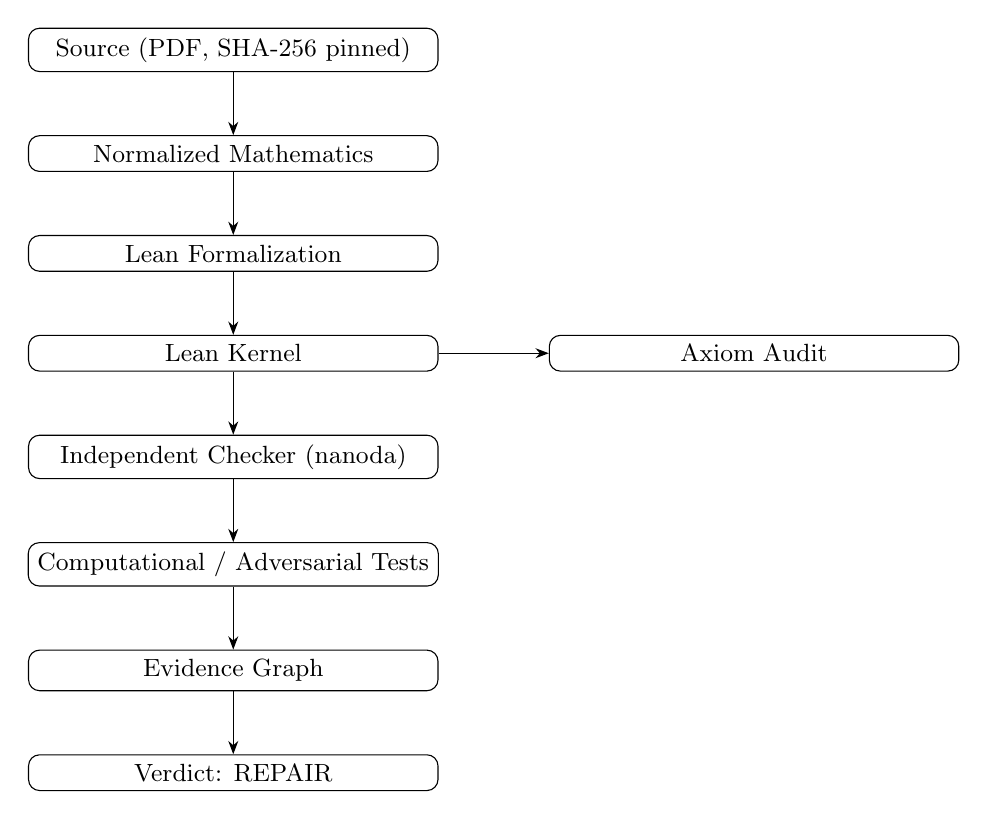
\begin{tikzpicture}[node distance=8mm, every node/.style={font=\small}, box/.style={draw,rounded corners,align=center,minimum width=52mm}, >=Stealth]
\node[box] (source) {Source (PDF, SHA-256 pinned)};
\node[box, below=of source] (norm) {Normalized Mathematics};
\node[box, below=of norm] (lean) {Lean Formalization};
\node[box, below=of lean] (kernel) {Lean Kernel};
\node[box, below=of kernel] (indep) {Independent Checker (nanoda)};
\node[box, below=of indep] (comp) {Computational / Adversarial Tests};
\node[box, below=of comp] (ev) {Evidence Graph};
\node[box, below=of ev] (verdict) {Verdict: REPAIR};
\node[box, right=14mm of kernel] (axiom) {Axiom Audit};
\draw[->] (source) -- (norm);
\draw[->] (norm) -- (lean);
\draw[->] (lean) -- (kernel);
\draw[->] (kernel) -- (axiom);
\draw[->] (kernel) -- (indep);
\draw[->] (indep) -- (comp);
\draw[->] (comp) -- (ev);
\draw[->] (ev) -- (verdict);
\end{tikzpicture}
\end{center}

\section{Reproducibility Instructions}
\begin{verbatim}
git clone https://github.com/tangentstorm/eliahou-collatz-bounds.git
cd eliahou-collatz-bounds
git checkout db804ce6305ea99a817f067869607f8b677d895a
lake exe cache get
lake build   # expect: Build completed successfully (8033 jobs)
\end{verbatim}
Reproducibility level: \textbf{R3} (formal verification reproducible; not yet R4).

\section{Correction Ledger}
See Appendix~C. One entry: a false ``mismatch'' from a float64 precision artifact in this audit's own adversarial test, caught before being trusted, root-caused, and corrected.

\section{Conclusion}
Every trust layer except independent (non-kernel) verification is fully satisfied for Eliahou's Theorem 1.1 as formalized in this repository, with the formalization's proof structure independently confirmed isomorphic to the source paper's own three-case Farey argument. The remaining gap is a specific, disclosed, root-caused tool limitation with defined repair paths --- not a defect in the mathematics. \textbf{Governance decision: REPAIR.}

\appendix
\section{Lean Source}
Full source: \texttt{Collatz/LinearForm.lean}, \texttt{Collatz/Defs.lean}, \texttt{Results.lean} in the cited repository/commit.

\section{Tests}
\texttt{verification/computational/tests/verify\_convergents.py} (this report's repository).

\section{Evidence Receipt}
Full verification receipt: \texttt{verification/receipt/verification-receipt.md}. Correction ledger: \texttt{verification/receipt/correction-ledger-entry.md} (two entries: a false-mismatch in the adversarial test, and a process-order deviation --- Report Generation was executed after, not before, the Governance Decision, reversed from Section~2's canonical chain; disclosed rather than silently reordered). Event ledger (hash-chained, 15 events): \texttt{verification/evidence/event-ledger.jsonl}, final event hash \texttt{7037245908c7ca08\ldots}, graph hash \texttt{0c9330331753c8b8\ldots}.

\section*{References}
\begin{enumerate}
\item Eliahou, S.\ (1993). The $3x+1$ problem: new lower bounds on nontrivial cycle lengths. \emph{Discrete Mathematics} 118(1--3), 45--56.
\item \texttt{tangentstorm/eliahou-collatz-bounds}, commit \texttt{db804ce6}.
\item \texttt{leanprover/lean4export}, \texttt{ammkrn/nanoda\_lib}.
\end{enumerate}

\end{document}
